%%__________________________________________________________________||
\section{Signal candidate event selection}
\label{sec:event_selection}

The event reconstruction and selection criteria described below are
explained in more detail in Ref.~\cite{RA1Paper2012}. In order to
suppress SM processes with genuine \ETmiss from neutrinos and select
only multijet final states, events containing an isolated
electron~\cite{PAS-EGM-10-004} or muon~\cite{PAS-MUO-10-004} with $\Pt
> 10\GeV$ or isolated photon~\cite{PAS-EGM-10-006} with $\pt > 25\GeV$
are vetoed. Furthermore, events containing an isolated track with $\Pt
> 10\gev$ are also vetoed in order to reduce the background
contribution from final states containing hadronically-decaying tau
leptons.

Jets are reconstructed using the particle-flow (PF) reconstruction
algorithm~\cite{CMS-PAS-PFT-09-001, CMS-PAS-PFT-10-001} and clustered
by the anti-$k_{\rm T}$ algorithm~\cite{antikt} with a size parameter
of $0.4$. The jet energies are corrected to account for the effects of
pileup and to establish a uniform relative response in $\eta$ and a
calibrated absolute response in transverse momentum
\pt~\cite{2011arXiv1107.4277C}. Jets considered in the analysis are
required to have a transverse energy above $40\gev$ and $|\eta| <
3$. The mass scale of the physics processes being probed is
characterised by the scalar sum of the transverse momenta $\Pt$ of
these jets, defined as $\scalht = \sum_{i=1}^{N_{\rm jet}}
\Pt^{\,\mathrm{j}_i}$, where $N_{\rm jet}$ is the number of jets
within the experimental acceptance. The estimator for \ETmiss is given
by the magnitude of the vector sum of the transverse momenta of these
jets, defined by $\mht = |\sum_{i=1}^{N_\text{jet}}
\ptvec^{\,\mathrm{j}_i}|$. Events are vetoed if rare, spurious signals
are identified in the calorimeters~\cite{1748-0221-5-03-T03014,
  CMS-NOTE-2010-012} or if any additional jet satisfies $\Pt > 40\GeV$
and $|\eta| > 3$, in order to maintain the performance of the variable
\mht as an estimator of \ETmiss.

Significant hadronic activity and \ETmiss in the event is ensured by
requiring $\scalht > 200\GeV$ and $\mht > 130\gev$, respectively. The
most energetic jet in the event is required to satisfy $\Pt >
100\gev$. A requirement on the second most energetic jet is used to
categorise the events. If the jet satisfies $\Pt > 100\gev$, then this
category of events is labelled ``symmetric'' and targets primarily the
topology of pair-produced sparticles. If the second most energetic jet
satisfies $40 < \Pt < 100\gev$ or $\Pt < 40\gev$, then these
categories are labelled as an ``asymmetric'' or ``monojet'' topology,
respectively. The final two topologies target primarily dark matter
and nearly mass-degenerate SUSY models. Events are further categorised
according to the number of jets per event (\njet) and the number of
reconstructed jets identified as originating from a b-quark (\nb).

A number of beam- and detector-related effects can lead to events with
large values of \ETmiss, such as beam halo, reconstruction failures,
spurious detector noise, or event misreconstruction due to detector
inefficiencies. These events, with large, non-physical values of
\ETmiss, are rejected with high efficiency by applying a range of
dedicated vetoes~\cite{RA1Paper2012, cms-met}.

\begin{table}[h!]
  \topcaption{Summary of the selection criteria and
    categorisation used in the definitions of the signal and control
    regions.} 
  \label{tab:selections}
  \centering
  \footnotesize
  \begin{tabular}{ ll }
    \hline
    \hline
%    Selection            & Details                                                                                            \\
%    \hline
    \multicolumn{2}{l}{\bf Baseline selection:}                                                                                \\
    Jets selection        & Select jets satisfying $\PT > 40\gev$ and $|\eta| < 3$                                             \\
    Forward jet veto      & Veto events containing jet satisfying $\PT > 40\gev$ and $|\eta| > 3$                              \\
    %Lepton/photon vetoes & $\PT > 10\gev$ and $|\eta| < 2.5$ for leptons, $\PT > 25\gev$ and $|\eta| < 2.5$ for photons       \\ 
    Lepton/photon vetoes  & $\PT > 10,\, 10,\, 25\gev$ for leptons, isolated tracks, photons (respectively) and $|\eta| < 2.5$ \\ 
    Lead jet acceptance   & $\PT > 100\gev$ and $|\eta| < 2.5$                                                                 \\
    Second jet acceptance & $\PT > 100\gev$ (symmetric), $40 < \PT < 100\gev$ (asymmetric), $\PT < 40\gev$ (monojet)           \\
    Energy sums           & $\scalht > 200\gev$ and $\mht > 130\gev$                                                           \\
    \ETmiss cleaning      & Various filters related to beam and instrumental effects                                           \\ 
    \hline
    \multicolumn{2}{l}{\bf (\njet,nb) categorisation and \scalht binning:}                                                     \\
    \njet binning         & 1 (monojet), 2, 3, 4, $\geq$5 (both symmetric and asymmetric)                                      \\
    \nb binning           & 0, 1, 2, $\geq3$ ($\nb \leq \njet$)                                                                \\
    \scalht (GeV) binning & 200, 250, 300, 350, 400, 500, 600, $>$800\gev (bins can be merged depending on \njet, \nb)         \\
    \hline
    \multicolumn{2}{l}{\bf Signal region:}                                                                                     \\
    QCD suppression       & $\alphat > 0.65$ to $\alphat > 0.52$ (\scalht-dependent, for the region $\scalht < 800\gev$)       \\
    QCD suppression       & $\bdphi > 0.5$                                                                                      \\
    QCD suppression       & $\mht/\ETmiss < 1.25$                                                                              \\
    \hline
    \hline
  \end{tabular}
\end{table}

For events satisfying the baseline selection criteria described above,
summarised in Table~\ref{tab:selections}, the multijet background
dominates over all other SM backgrounds. The \alphat kinematic
variable, first introduced in Refs.~\cite{Randall:2008rw, RA1Paper},
is used to efficiently reject multijet events with transverse energy
mismeasurements while retaining sensitivity to new physics with
genuine \ETmiss signatures. The variable \alphat depends solely on the
measurements of the transverse energies and azimuthal angles of jets
and it is intrinsically robust against the presence of jet energy
mismeasurements in multijet systems. For dijet events, the \alphat
variable is defined as $\alphat = \Et^{\rm j_2}/M_\text{T}$ where
$\Et^{\rm j_2}$ is the transverse energy of the less-energetic jet,
and $M_\text{T}$ is the transverse mass of the dijet system.  For a
perfectly measured dijet event with $\Et^{\mathrm{j}_1} =
\Et^{\mathrm{j}_2}$ and jets back-to-back in $\phi$, and in the limit
in which the momentum of each jet is large compared with its mass, the
value of \alphat is 0.5. For the case of an imbalance in the measured
transverse energies of back-to-back jets, \alphat is reduced to a
value smaller than 0.5, which gives the variable its intrinsic
robustness. Values significantly greater than 0.5 are observed when
the two jets are not back to back and are recoiling against
significant, genuine \ETmiss. The definition of the \alphat variable
can be generalised for events with two or more jets, as described in
Ref.~\cite{RA1Paper2012}.

Multijet events typically populate the region $\alphat \lesssim 0.5$
and the \alphat distribution is characterised by a sharp edge at 0.5,
beyond which the multijet event yield falls by several orders of
magnitude. Multijet events with extremely rare but large stochastic
fluctuations in the calorimetric measurements of jet energies can lead
to values of \alphat slightly above 0.5. The edge at 0.5 sharpens with
increasing \scalht for multijet events, primarily due to a
corresponding increase in the average jet energy and thus an
improvement in the jet energy resolution, but also because the
threshold effect of jets below the \Pt threshold contributing
significantly to \mht decreases with increasing \scalht. This
motivates a \scalht-dependent \alphat requirement that varies in the
range 0.52--0.65 for the region $\scalht < 800\gev$. 
%For the region $\scalht > 800\gev$, the necessary control of the QCD
%multijet background is achieved solely with the \bdphi variable.

%Two further dedicated event vetoes are employed to suppress the QCD
%multijet background to a negligible level. 
The \bdphi variable considers the minimum azimuthal angular separation
of a jet and the \mht vector derived from all other jets in the
event. The \bdphi variable provides powerful discriminating power
between final states with genuine \ETmiss and mismeasured QCD multijet
events. The variable is also highly efficient at suppressing any
potential contribution from rare energetic multijet events that yield
high jet multiplicities and significant \ETmiss due to
high-multiplicity neutrino production in semileptonic heavy-flavour
decays. The neutrinos are typically collinear with respect to the axis
of a jet and carry a significant fraction of the energy. The
requirement $\bdphi > 0.5$ is sufficient to suppress effectively the
multijet background.

For the region $\scalht < 800\gev$, the requirements on both the
\alphat and \bdphi variables are utilised, whereas for the region
$\scalht > 800\gev$, the necessary control of the QCD multijet
background is achieved solely with the \bdphi
requirement. Figure~\ref{fig:alphat-bdphi} shows the \alphat and \bdphi
distributions observed in data for events that satisfy all other
signal region selection criteria plus $\scalht > 300\gev$ and $\scalht
> 800\gev$, respectively. In the case of the \alphat distribution, the
events that satisfy $\alphat < 0.55$ must only fulfill the baseline
selection criteria defined in Table~\ref{tab:selections}, no \mht
requirement is made, and the events are recorded with an unbiased set
of trigger \scalht conditions.

\begin{figure*}[tbhp]
  \begin{center}
    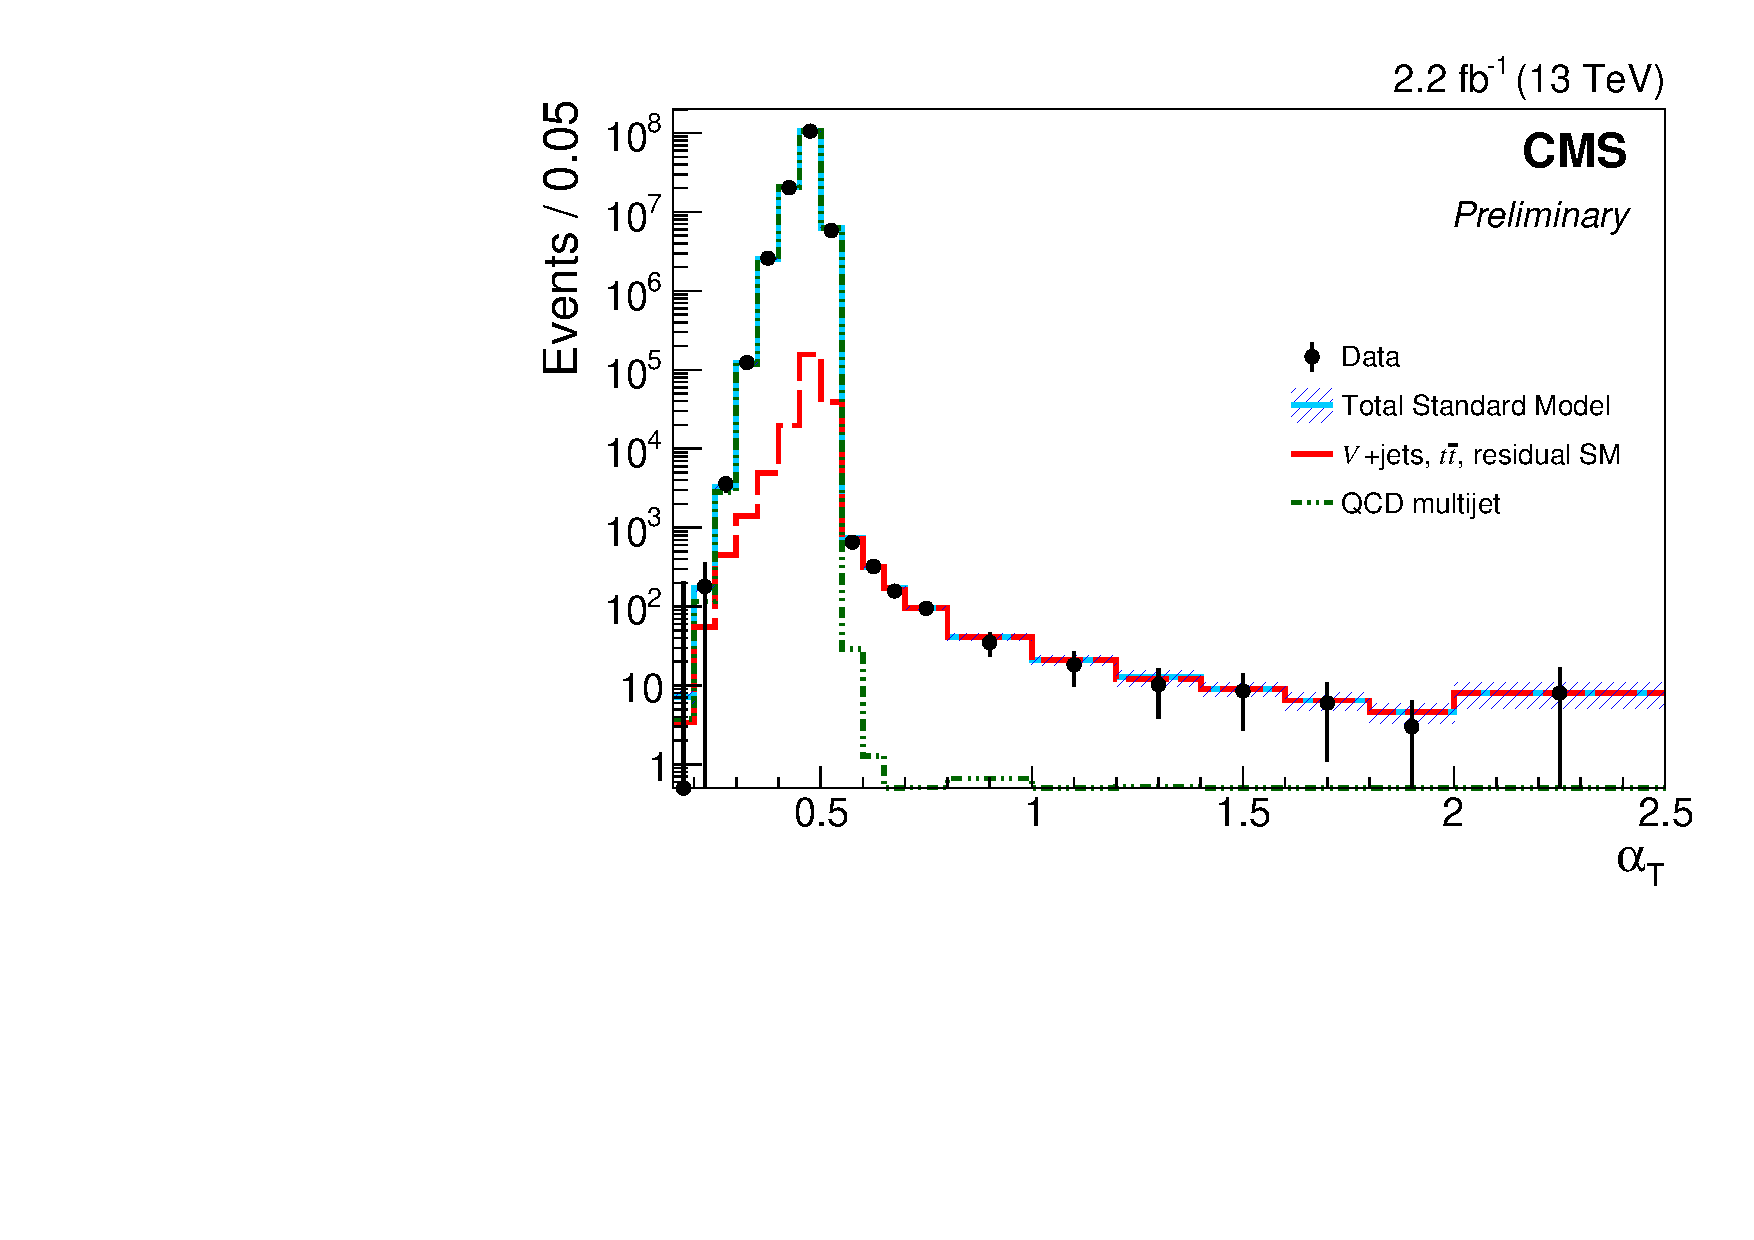
\includegraphics[width=0.49\textwidth]{alphaT_v4} \,
    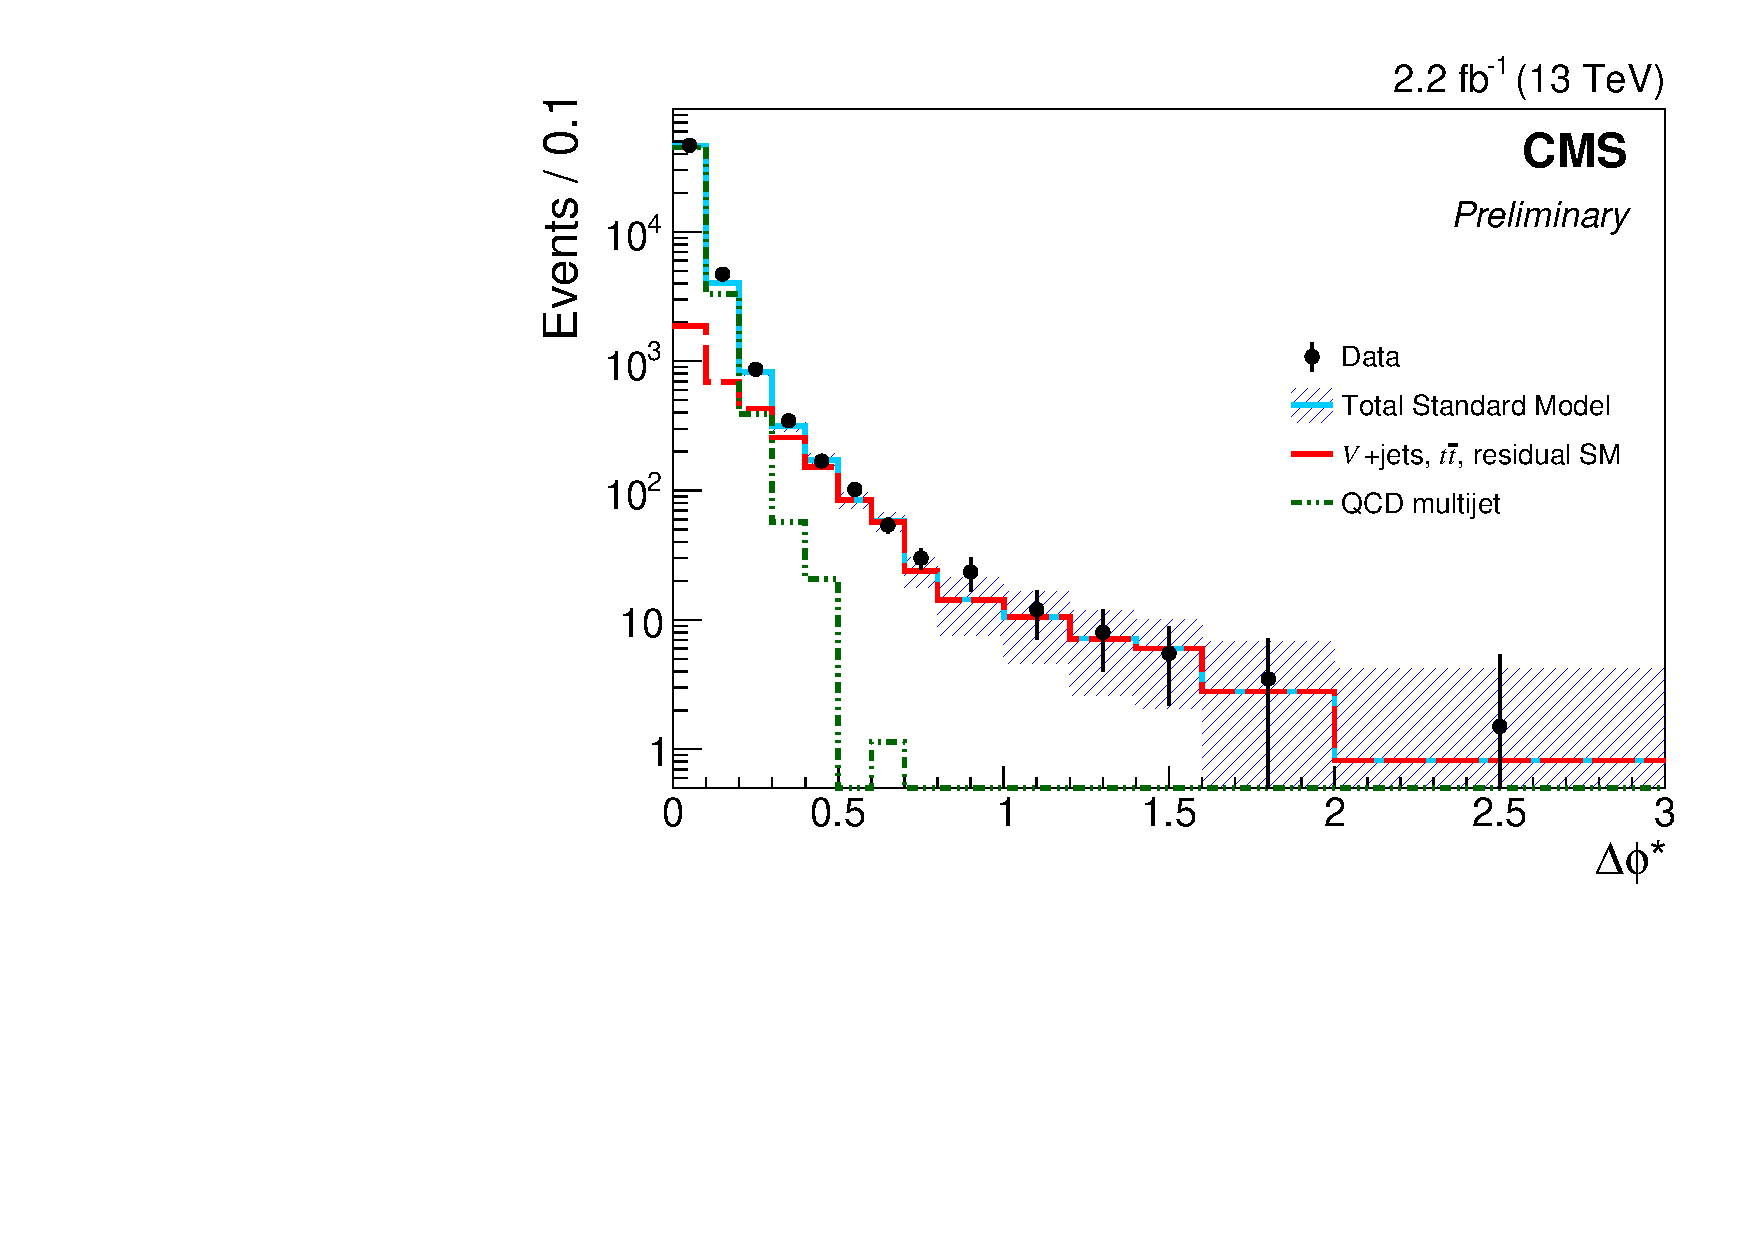
\includegraphics[width=0.49\textwidth]{bDPhi_v4} \\
  \end{center}
  \caption{(Left) The \alphat distribution observed in data for events
    that are recorded with unbiased trigger conditions and satisfy the
    baseline (full signal region) selection criteria for the region
    $\alphat < 0.55$ ($\alphat > 0.55$). (Right) The \bdphi
    distribution observed in data for events that satisfy the full
    signal region selection criteria and $\scalht > 800\gev$.  The
    distributions for the QCD multijet backgrounds are determined from
    simulation while all other SM backgrounds are estimated using a
    $\mu$ + jets data control sample. %The uncertainties in the SM
    %expectation are dominated by the statistical uncertainties 
    %associated with the limited sample of simulated multijet events.
    \label{fig:alphat-bdphi} 
  }
\end{figure*}

%Two further dedicated event vetoes are employed to suppress the QCD
%multijet background to a negligible level. The first veto is based on
%the aforementioned \bdphi variable, which considers the minimum
%azimuthal angular separation of a jet and the \mht vector derived from
%all other jets in the event. This variable is employed to suppress any
%potential contribution from rare energetic multijet events that yield
%high jet multiplicities and significant \ETmiss due to
%high-multiplicity neutrino production in semileptonic heavy-flavour
%decays. The neutrinos are typically collinear with respect to the axis
%of a jet and carry a significant fraction of the energy. The
%requirement $\bdphi > 0.5$ has been demonstrated with a data control
%sample to suppress effectively this background source.

%The second veto concerns ...
A final dedicated veto is employed to deal with the rare circumstance
in which several jets with transverse energies below the \Et
thresholds and collinear in $\phi$ can result in significant \mht
relative to \ETmiss, the latter of which is less sensitive to jet
thresholds. This type of background, typical of multijet events, is
suppressed while maintaining high efficiency for SM or new physics
processes with genuine, significant missing transverse momentum by
requiring $\mht / \ETmiss < 1.25$. 

The aforementioned requirements complete the definition of the signal
region. Signal candidate events are recorded with multiple jet-based
trigger conditions that require both \scalht and \alphat to satisfy
predetermined thresholds. In addition, a trigger condition based
solely on \scalht is used to record candidate events for
the region $\scalht > 800\gev$. A dedicated trigger condition
comprising the presence of a jet and significant \mht and \ETmiss is
used to record monojet events. The trigger-level jet energies are
corrected to account for energy scale and pileup effects. The trigger
strategy provides efficiencies at or near 100\% for all bins of the
signal region.

Finally, the search exploits the use of the \mht variable as a
discriminant between the dominant SM backgrounds and new physics
signatures. The \mht templates are derived from simulation that are
extensively validated in multiple data control regions and from which
systematic uncertainties are established.
